\specialsection{Community}{}{white}{black}

\begin{figure}
	\centering
	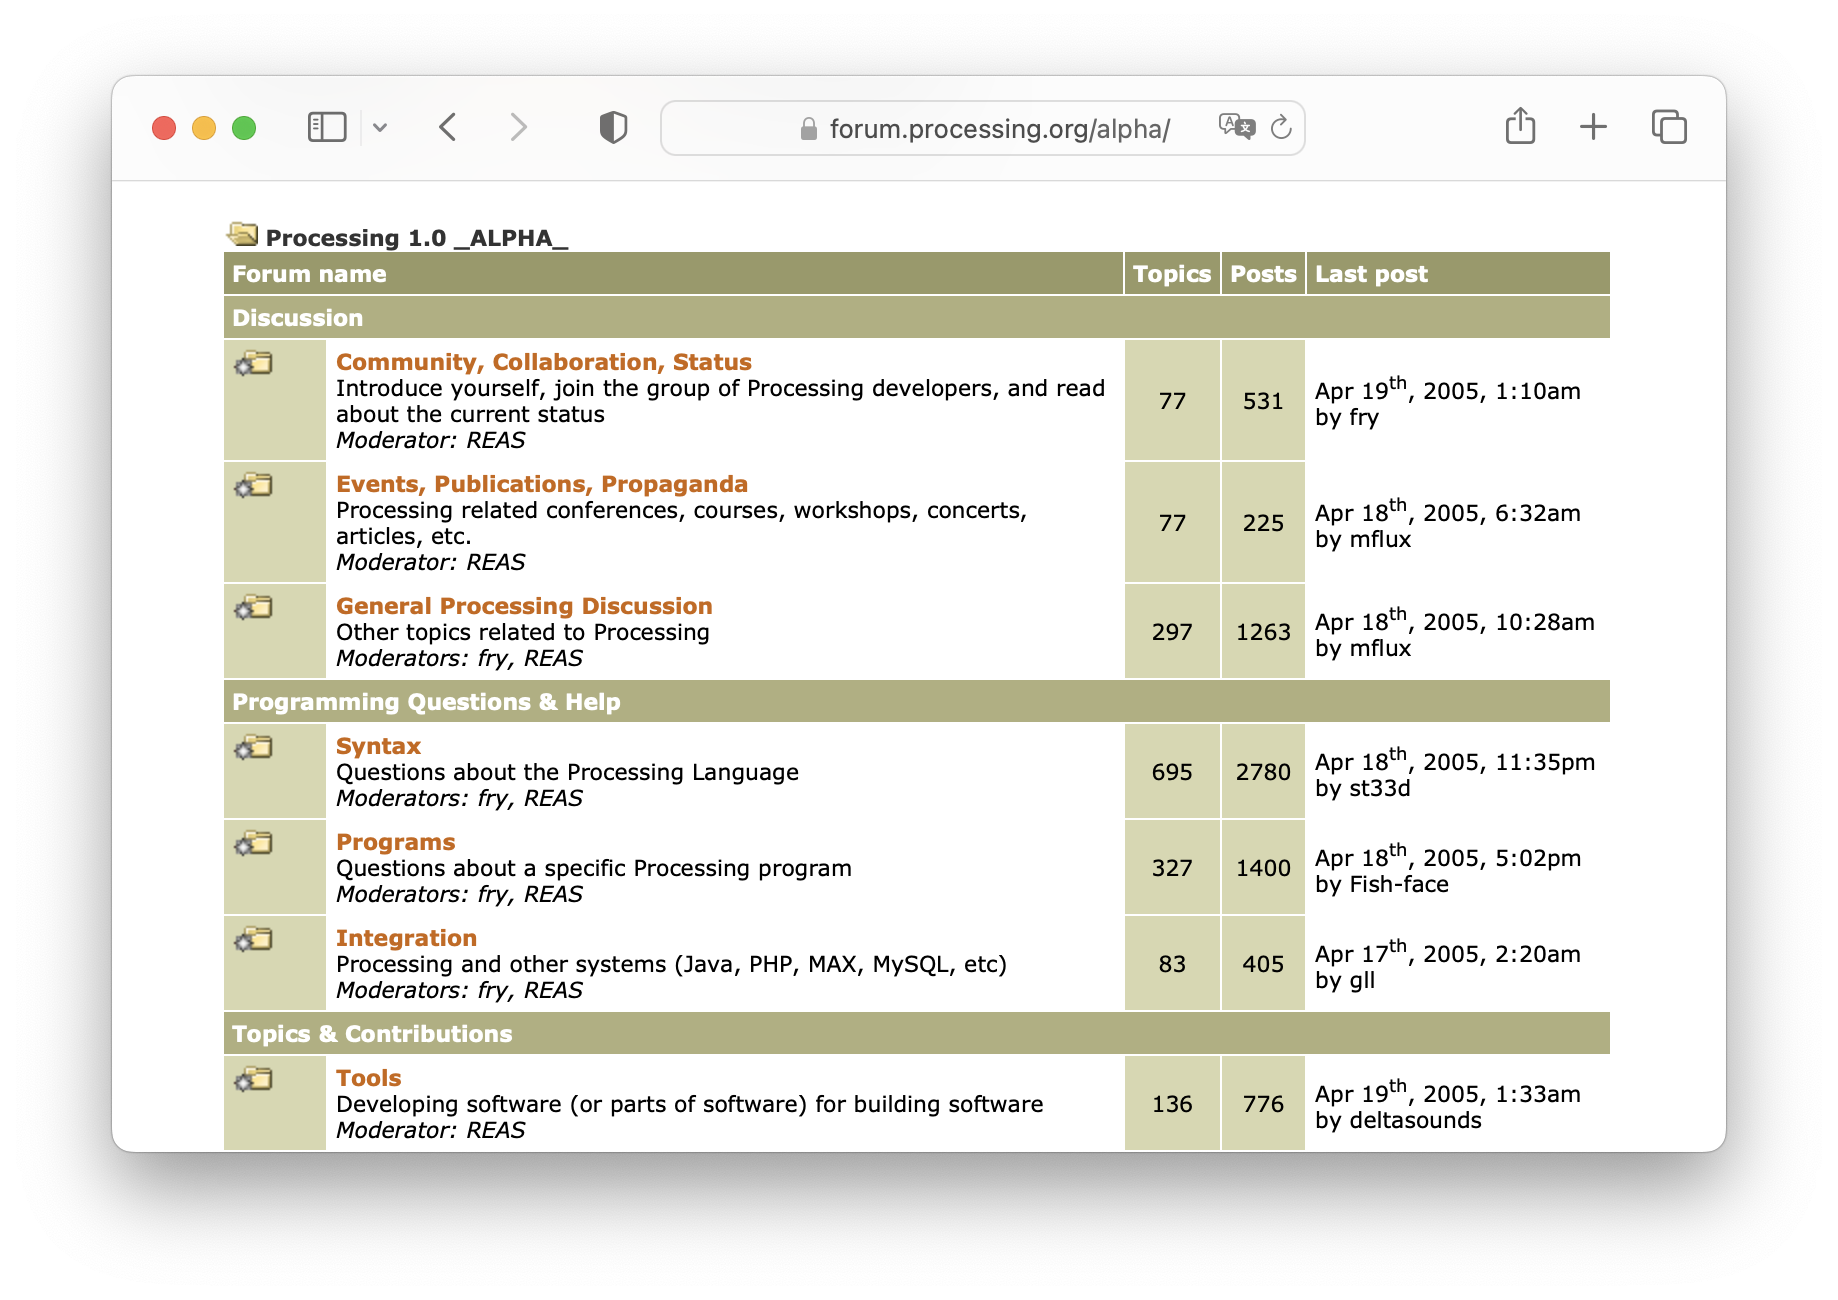
\includegraphics[width=1.0\textwidth]{images/alpha-browser.png}
	\caption{Screenshot of the Processing Alpha Forum}
	\label{fig:processing-alpha}
\end{figure}

\subsection{A Community of Practice}
It is vital to acknowledge that software development encompasses more than just the technical aspects of the project. Understanding the interactions and dynamics within the community is just as crucial. The Processing community, for example, values various valuable ways to contribute beyond writing code, such as teaching, organizing events, and creating tutorials and documentation. Some contributors even consider end-users as contributors as they provide the reason and purpose for developing and teaching software \parencite[41]{processingfoundation20thAnniversaryProcessing2022}. 

Wenger’s Communities of Practice \parencite{wengerCommunitiesPracticeLearning1998} theoretical framework was employed in our analysis to understand these additional relationships further. This model is particularly relevant, given that the focus on education and the dynamics of the early Processing community portray an informal learning organization. The early community succeeds in peer-to-peer interaction, collaborative discussions, and shared creative exploration. These characteristics align closely with the three prevalent fundamental elements of Wegner’s model: mutual engagement, joint enterprise, and shared repertoire, but they also incorporate less discussed concepts like legitimate peripheral participation. 

Mutual Engagement refers to the collaborative interaction and relationships within the community, where members actively participate, share knowledge, and support each other. Joint Enterprise is the collective goal or endeavor that unites the community, providing a shared purpose and direction for its activities. Shared Repertoire encompasses the range of communal resources - tools, language, stories, and practices - developed over time, which embody the community’s collective knowledge and cultural identity. These elements foster a dynamic, collaborative environment that promotes learning and knowledge sharing.

The forthcoming analysis seeks to delineate and interpret the identified elements, employing the Communities of Practice framework as a guiding lens. This methodological choice is advantageous, given the diverse identified dynamics and relationships. Furthermore, the application of this model not only facilitates an analysis of the evolution of these elements over time but can yield insights into the broader implications of community-led software development and learning.

At the beginning of the Processing project, the alpha forum was the community’s central means of exchange. As asserted by Reas, the forum cultivated a ’unified international community’ from 2002 to 2006 \parencite[331]{conradGraphicDesignPostdigital2021}.

As such, the forum was subjected to data scraping and analysis to identify the most engaged members based on their posting activity. The three most active participants, apart from the project’s co-creators, Ariel Malka, Martin Gomez, and Jacob Schwartz, were interviewed. 

The chapter begins with an analysis of the integration of this particular group into the community, followed by a broader examination of community dynamics in general.


\cleardoublepage
\changepapersize{305.3mm:210mm}
\customtag{largepage}
{
	\LARGE
	\noindent Alpha Forum Top Contributors\par
	\vspace{0.2cm} 
}
\vfill

\begin{figure}[h!]
	\centering
	\frame{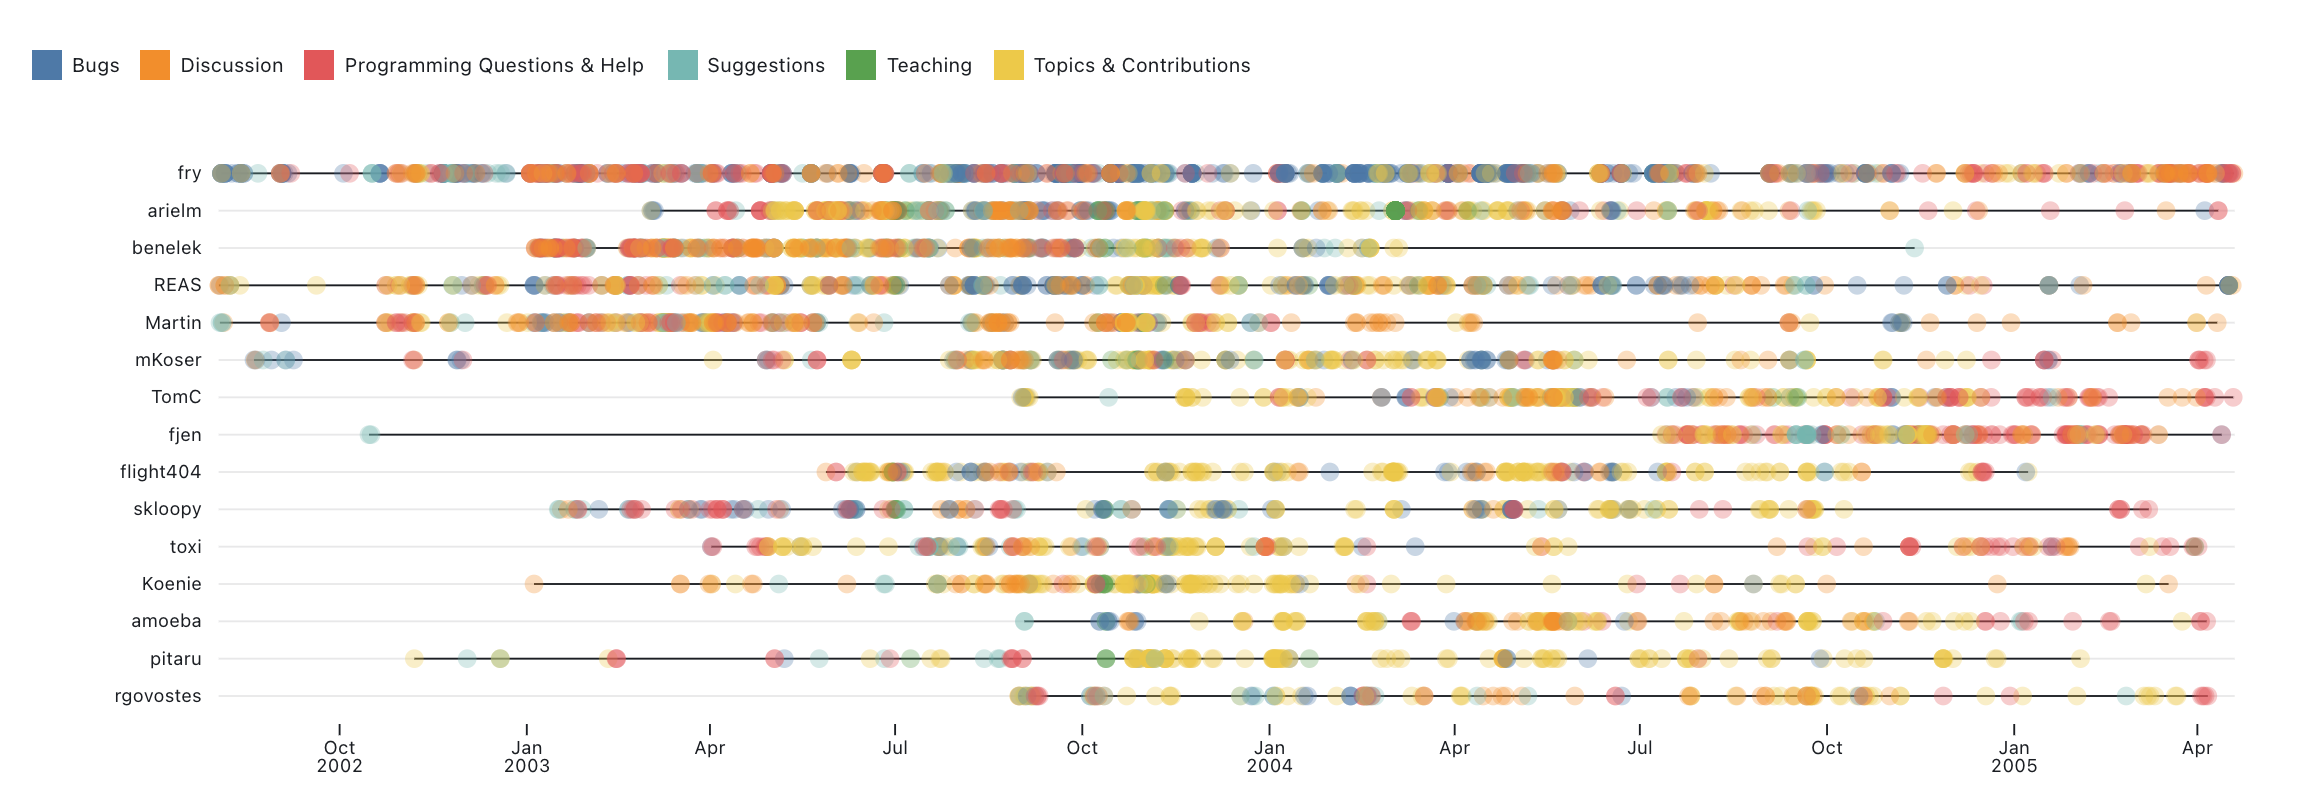
\includegraphics[width=1.0\textwidth]{images/alpha-forum-top15.png}}
	\caption{Posting activity of the 15 most active contributors on the alpha forum.}
	\label{fig:processing-alpha-dot}
\end{figure}

% Add commentary to the graph
\begin{multicols}{3}
	\noindent
  Figure \ref*{fig:processing-alpha-dot} shows a timeline of color coded post by category of the 15 most active contributors to the Alpha forum. Among them Ariel Malka (arielm), Jacok Schwartz (benelek) and Martin Gomez (Martin) were interviewed, on the basis of their participation in the forums, with no definitive indications of them assuming additional roles such as library contributor. We can observe certain patterns emerging such as initial posts being often in the Programing Help \& Questions section, often spanning out to others in the future. A part from co-creators Ben Fry (fry) and Casey Reas (REAS) we can also observe clustering of posts for users, suggesting periods of activity and inactivity. 
  \columnbreak

  \vfill\null
\end{multicols}
\defaultareasettings

\begin{table}[h]
	\raggedright
	\begin{adjustbox}{center}
		\begin{tabular}{l l l c}
			\toprule
			Forum name                   & Years      & URL                                                                    \\
			\midrule
			Processing alpha forum       & 2002-2005  & \href{https://forum.processing.org/alpha/}{forum.processing.org/alpha} \\
			Processing beta forum        & 2005-2010  & \href{https://forum.processing.org/beta/}{forum.processing.org/beta}   \\
			Processing 1.0 forum         & 2010-2013  & \href{https://forum.processing.org/one/}{forum.processing.org/one}     \\
			Processing 2.0 and 3.0 forum & 2013-2018  & \href{https://forum.processing.org/two/}{forum.processing.org/two}     \\
			Current processing forum     & 2018 - now & \href{https://discourse.processing.org/}{discourse.processing.org}     \\
			\bottomrule
		\end{tabular}
	\end{adjustbox}
	\caption{Archival forums composition}
	\label{table:forums}
\end{table}

\subsection{Forum Contributors}

Within the Processing forums, the evolution from newcomer to integral community member exemplifies Wenger’s notion of legitimate peripheral participation  \parencite[117]{wengerCommunitiesPracticeLearning1998}. This concept describes how individuals initially engage at the community’s margins and, through increased involvement, move toward a more involved role. Ariel Malka, Martin Gomez, and Jacob Schwartz are case studies of this journey as they navigated from the outskirts to significant presence, carving out their professional identities without local counterparts in computational design.

Initially, these individuals engaged primarily in observing and learning from the exchanges of others. Interviewees mentioned reading and getting inspired by various technical discussions, such as how to simulate physical hair models by other users, such as Karsten Schmidt, or being impressed by the work of other forum participants, such as Glen Murphy. This observational phase is crucial in legitimate peripheral participation, allowing individuals to acclimate to the community norms, language, and practices.

Figure~\ref{fig:processing-alpha-dot} shows the transitional phase as participants move from observers to active forum contributors. The friendly atmosphere of the forums has facilitated this transition, as we can observe the participants shifting their focus from \enquote{Programming Questions and Help}related topics to more vast topics. This positive environment is unlike the often confrontational atmospheres of other online forums, which can be daunting for new posters. Gomez found the processing forums to be a conducive environment for learning, where experienced users were always willing to help and point new users in the right direction, as he said: \enquote{In the processing forums, I never encountered things like that. They would always assume that you are there to learn and (...) they would usually just point you in the proper direction and be able to help you out}.

Schwartz’s words also capture the essence of evolving involvement: \enquote{I got a lot out of posting what I was working on and then getting feedback from that and looking at what other people were working on and seeing how they did those things}. This reflection highlights his transition from passive observation to active contribution and underscores the reciprocal nature of learning within the community. By sharing his work, receiving feedback, and drawing inspiration from others, Schwartz moved from the periphery of the community towards a more central, contributory role.

Similarly, Ariel Malka and Martin Gomez’s narratives reflect this transformative community engagement. Malka got involved more profoundly and transitioned from basic forum participation to contributions, such as participating in community exhibitions and testing software. Gomez, who felt isolated in his home country’s computational design domain, found a vital platform for development and collaboration in the Processing forum, moving from a solo enthusiast to an active community contributor. He pointed out that he was later able to create the first exhibitions in the Philippines relating to computational design.

These narratives collectively illustrate how online platforms, like the Processing forums, serve as critical enablers for legitimate peripheral participation. They provide a conduit for individuals without local communities to engage, learn, and contribute meaningfully. 

The experiences of Malka, Gomez, and Schwartz not only shed light on the practical application of this concept but also underscore the importance of digital communities in nurturing individual growth, fostering skill development, and establishing a sense of belonging within specialized fields.


\newpage
\begin{figure}
	\centering
	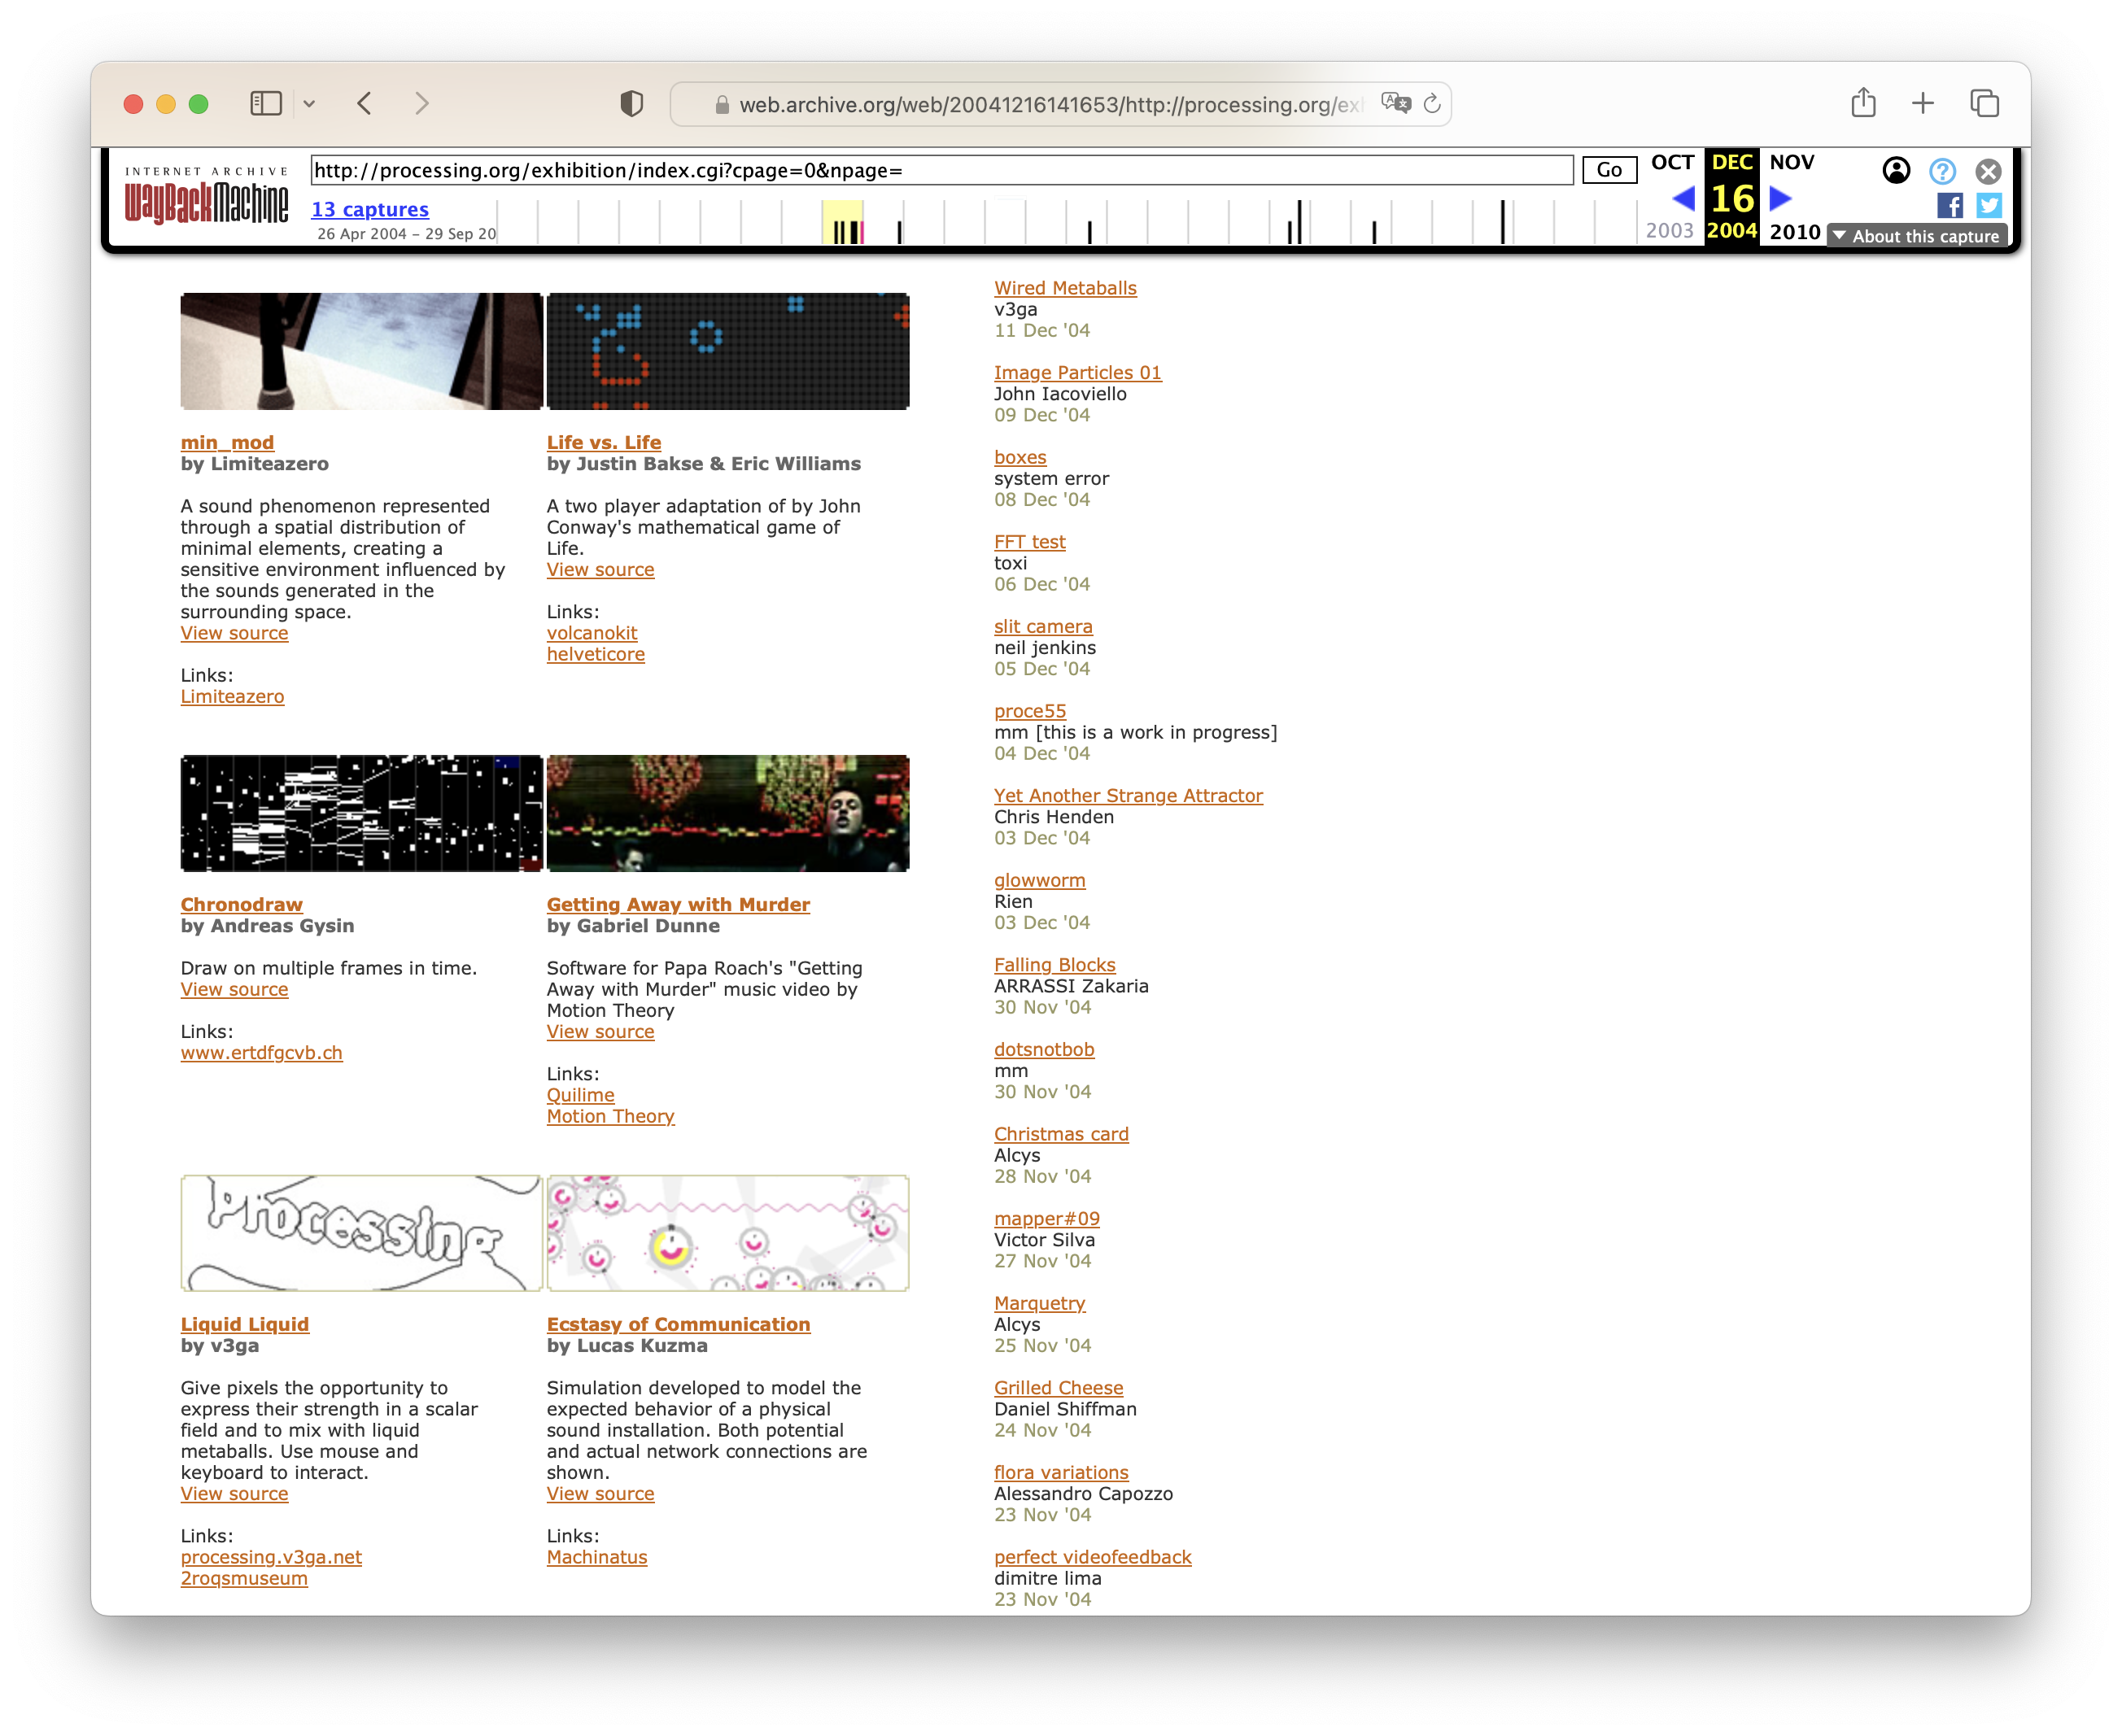
\includegraphics[width=1.0\textwidth]{images/exhibitions.png}
	\caption{Screenshot of community exhibition}
	\label{fig:website-exhibition}
\end{figure}

\subsection{Community Dynamics}
The Processing distinguishes itself by appreciating commonly overlooked \enquote{community maintenance} activities such as creating examples, writing documentation, and organizing exhibitions. As Wenger points out, these are intrinsic parts of the practice but are usually much less visible than instrumental parts, in the case of Processing releasing a new version of the IDE, for instance. \parencite[78]{wengerCommunitiesPracticeLearning1998}

Through the proce55ing.net website, the community has strongly emphasized sharing concise prototypical code examples that illustrate a feature or concept. This trait was already present in the first version of the website, which only included an index, examples, and reference pages. By establishing these norms and best practices early on, newcomers could embrace and propagate these shared standards, contributing to the shared repertoire of the group. 

While the example projects showcased the basics, the exhibition page featured more significant works. The co-founders of Processing, Ben Fry and Casey Reas shared their work, Valence and Tissue, which set a standard and expectation for others to follow. Other community members were encouraged to participate, resulting in similar works of similar scope. The source code for all of these works was made available, making the exhibition a showcase of projects and a learning opportunity for the community.

These methods create a low barrier to entry through examples and a high ceiling by sharing more consequential works. As noted by Fry, the project showcases would attract new members to the forums: \enquote{With each person who created something there, we would see an uptick of people participating in the forum who were followers of that person’s work}.

The project saw increased user engagement thanks to its features facilitating the onboarding of new users and community members. The website presentation effectively showcased the shared repertoire, which encouraged users to become active participants in the community of practice.

These efforts were exploratory. Schmidt points out that the initial community shared a common goal of exploration. \enquote{In the beginning, it was a small group, and everyone was learning together what this thing is, or what it could do}, he notes, highlighting the joint enterprise of the whole community. The software’s development can be seen as an artifact of this joint enterprise. It embodied the community’s learnings from experimentation as a whole. It featured an evolutionary process influenced by the development of libraries, which were the outcomes of earlier experiments.

The term \enquote{processing} itself evokes computational and artistic processes involving iterating through variations. In this community, it is primarily associated with software sketching, but it can be applied to the community as a whole. People in the forums discuss various topics such as Information Visualization, Simulation, Artificial Life, and more. 
The community’s direction, shaped through these vibrant discussions and experiments, resonates with Wenger’s CoP principles. As Schmidt pointed out, people at the time were thinking, \enquote{Perhaps the tool can be modified in the future to make these things more possible}. This reflects the CoP’s core aspect of dynamic meaning negotiation. This continual dialogue and experimentation within the community are emblematic of the learning and communal development emphasized in Wenger’s framework.

Moreover, the community’s engagement extends beyond technical aspects to philosophical debates, further illustrating the CoP’s concept of shared meaning creation. Discussions in the forums, debating the intersections of code, design, and art, exemplify this. Topics such as \enquote{code != art} or \enquote{Processing = Design? Art? Other?} generate substantial interaction and highlight the community’s diverse perspectives on project priorities. These debates, sometimes questioning the project’s inclusivity towards artists and designers, underscore the ongoing process of negotiating meaning and priorities, a fundamental element in Wenger’s CoP framework.

The richness of the community’s engagement was only possible with the mutual engagement of forum participants and the formation of relationships between them.  Interviewees often mentioned other users from whom they learned, as Jacob Schwartz notes, for example, \enquote{I still remember some of these usernames here. I was so impressed with Glen Murphy’s projects}. 

It was common for experienced individuals like Murphy to share their work-in-progress posts, even on complex subjects such as Fluid Dynamics. For instance, on November 5th, 2002, he shared two code examples and the message \enquote{Neither of these are ’full’ fluid simulations. For example, Navier-Stokes is nowhere to be seen, and the pressure calculations are pretty raw. May be useful as a base for something}. This highlights the importance of giving back, inviting feedback and conversation, and integrating the learning process. This approach contrasts with solely sharing work to impress peers or showcasing finished products only.

Reflecting on his experience, Schwartz emphasized the significance of the community in addition to the tool, stating, \enquote{I would say that the tool itself was very interesting to me, but the community was a huge part of it for me as well}. This perspective emphasizes the value placed on the initial community, implying a collective responsibility for the community.

Schmidt builds on this notion, focusing on the community aspect of open-source projects. He articulates the implicit social contract involved in using open-source tools, which entails actively participating in the community. Schmidt explains, \enquote{When you sign up to use open source tooling, you make a kind of social agreement to be part of that culture, which gives you so much that there should be a social expectation also to want to give something back}.

Marxer adds to this topic by highlighting the responsibility he felt towards users of his library. Reflecting on user interactions, he notes, \enquote{Every time that somebody would use it or would point out maybe some mistake, you said, ’Oh, then people are relying on this.’ So you try to fix the mistake and put it into the next version}. This perspective emphasizes the dynamic relationship between users and community participants, where feedback leads to continuous improvement and engagement.

The combination of community dynamics has created a positive feedback loop that engages users. The exhibition’s potential draws them in, and they quickly start experimenting with different examples. They actively participate in the forum and gradually become community members by making diverse contributions. Measurable data such as forum activity and software usage statistics confirm this success. According to the Processing Foundation, over 250,000 unique users utilize Processing monthly.

As the project grew and matured, there was a noticeable shift in the community’s dynamics and user perceptions. Schmidt pointed out that the Processing community has undergone a cultural shift where contributions are now sometimes viewed more as products rather than collaborative efforts. This indicates a disconnection from the shared repertoire and mutual engagement that once surrounded the original alpha forum. Compared to before, typical users integrate less into the ecosystem.

There is a viewpoint that the project has matured, and due to its widespread adoption, community participation in developing the tool is no longer considered necessary. As the project’s primary goal has shifted towards educating novices in computer literacy, the joint exploration of computational design needs to be re-addressed. As a result, the tool’s usage has increased, but the dynamics have shifted away from being a community of practice, especially in the official discussion forums.

\begin{figure}
    \centering 
    \includesvg[pretex=\sffamily\fontsize{5.58pt}{8pt}\selectfont, width=1\textwidth, keepaspectratio]{images/alpha-forums-by-posts.svg}
    \caption{Topics by post number}
    \label{fig:forums}  
  \end{figure}

This shift from a general interest in computational design towards a more tool-centric approach is reflected in the current organization of the processing forum, which does not prioritize main categories such as automated systems, tangible computing, or artificial life. Instead, the forum is organized based on software flavors, including p5.js, Processing, Processing for Android, etc.

In sum, the early community exemplifies Etienne Wenger’s principles of mutual engagement, joint enterprise, and shared repertoire in a community of practice. This group, driven by a unified enthusiasm for computational design, created a collaborative environment where members exchanged knowledge, experiences, and resources. Their concerted efforts to develop and enhance the  platform underscored a collective goal, fostering technical skill advancement and philosophical discussions. This interaction resulted in a comprehensive repository of communal assets, signifying a successful, cooperative, and productive community. Although the dynamics of this project have evolved, its foundational success and growth can be attributed to these elements.


\cleardoublepage
\changepapersize{305.3mm:210mm}
\customtag{largepage}
% \fancyhf{} % Clear all header and footer fields


% \setlength{\spiralWidth}{10.7mm}
% 147.3
\begin{minipage}{147.3mm}
{
	\LARGE
	\noindent Community Connectedness \par
}
\begin{figure}[H]
	\centering
	\includesvg[pretex=\sffamily\fontsize{5.58pt}{8pt}\selectfont, width=0.95\textwidth, keepaspectratio]{images/year.svg}
	\caption{Connectedness through forum threads of top 100 alpha forum contributos}
	\label{figure:year}
\end{figure}

\end{minipage}

\newpage
% \pagestyle{fancy}

\customtag{largepage}
\begin{minipage}[t]{0.7\textwidth}
\begin{figure}[H]
  \begin{adjustbox}{width=\textwidth, keepaspectratio}
      \begin{tabular}{cccc}
          % Row 1
          \begin{subfigure}[b]{0.24\textwidth}
              \centering
              \includesvg[width=\linewidth, keepaspectratio]{images/month1.svg}
              \caption{Month 1}
              \label{fig:month1}
          \end{subfigure} &
          \begin{subfigure}[b]{0.24\textwidth}
              \centering
              \includesvg[width=\linewidth, keepaspectratio]{images/month2.svg}
              \caption{Month 2}
              \label{fig:month2}
          \end{subfigure} &
          \begin{subfigure}[b]{0.24\textwidth}
              \centering
              \includesvg[width=\linewidth, keepaspectratio]{images/month3.svg}
              \caption{Month 3}
              \label{fig:month3}
          \end{subfigure} &
          \begin{subfigure}[b]{0.24\textwidth}
              \centering
              \includesvg[width=\linewidth, keepaspectratio]{images/month4.svg}
              \caption{Month 4}
              \label{fig:month4}
          \end{subfigure} \\
          % Row 2
          \begin{subfigure}[b]{0.24\textwidth}
              \centering
              \includesvg[width=\linewidth, keepaspectratio]{images/month5.svg}
              \caption{Month 5}
              \label{fig:month5}
          \end{subfigure} &
          \begin{subfigure}[b]{0.24\textwidth}
              \centering
              \includesvg[width=\linewidth, keepaspectratio]{images/month6.svg}
              \caption{Month 6}
              \label{fig:month6}
          \end{subfigure} &
          \begin{subfigure}[b]{0.24\textwidth}
              \centering
              \includesvg[width=\linewidth, keepaspectratio]{images/month7.svg}
              \caption{Month 7}
              \label{fig:month7}
          \end{subfigure} &
          \begin{subfigure}[b]{0.24\textwidth}
              \centering
              \includesvg[width=\linewidth, keepaspectratio]{images/month8.svg}
              \caption{Month 8}
              \label{fig:month8}
          \end{subfigure} \\
          % Row 3
          \begin{subfigure}[b]{0.24\textwidth}
              \centering
              \includesvg[width=\linewidth, keepaspectratio]{images/month9.svg}
              \caption{Month 9}
              \label{fig:month9}
          \end{subfigure} &
          \begin{subfigure}[b]{0.24\textwidth}
              \centering
              \includesvg[width=\linewidth, keepaspectratio]{images/month10.svg}
              \caption{Month 10}
              \label{fig:month10}
          \end{subfigure} &
          \begin{subfigure}[b]{0.24\textwidth}
              \centering
              \includesvg[width=\linewidth, keepaspectratio]{images/month11.svg}
              \caption{Month 11}
              \label{fig:month11}
          \end{subfigure} &
          \begin{subfigure}[b]{0.24\textwidth}
              \centering
              \includesvg[width=\linewidth, keepaspectratio]{images/month12.svg}
              \caption{Month 12}
              \label{fig:month12}
          \end{subfigure}
      \end{tabular}
  \end{adjustbox}
  \caption{First year of the Alpha forum}
  \label{fig:monthlyGraphs}
\end{figure}
\end{minipage}
\hfill
\begin{minipage}[t]{0.25\textwidth}
  \vspace{8mm}
  \small
  The Alpha forum's developmental trajectory over its first year, as visualized through network graphs, reveals a dynamic growth narrative. Initially, a compact hub of activity signals robust engagement from a committed group of participants, laying the groundwork for the community's expansion. This is evidenced by an increase in the density and reach of interactions, suggesting a broadening in the diversity of contributors and a rise in active membership. The persistent complexity of the network and uniform distribution of connections throughout the year highlight an environment where individuals are actively integrated, promoting a collective and inclusive exchange of knowledge.

  \medskip
  The absence of isolated clusters within these visualizations speaks to a forum culture that successfully assimilates newcomers into the ongoing dialogue, maintaining an equitable and collaborative discourse. This enduring interactivity, underscores the forum's efficacy as a thriving digital ecosystem conducive to sustained collaboration and exchange.

\end{minipage}

\defaultareasettings

%\begin{figure}[h!] 
    \centering 
    \includesvg[pretex=\sffamily\fontsize{5.58pt}{8pt}\selectfont, width=1\textwidth, keepaspectratio]{images/figure-forum-posts.svg}
    \caption{Top 12 authors by number of posts (Aggregated alpha and beta forum)}
    \label{fig:forum-posts}  
  \end{figure}
%\begin{figure}[htbp] 
    \centering
    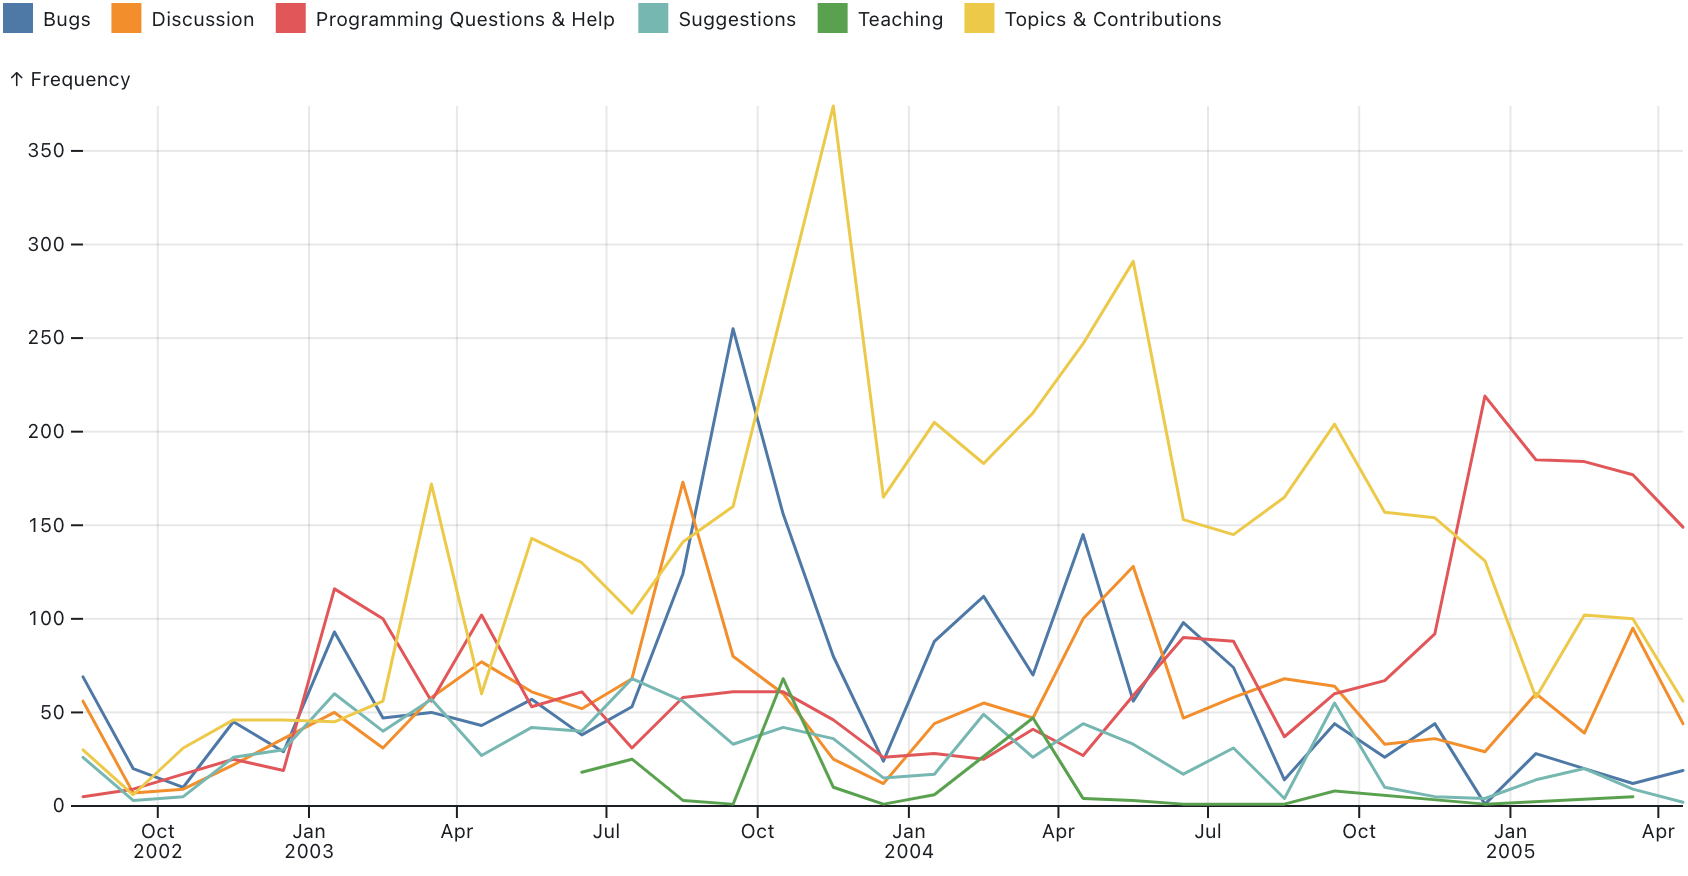
\includegraphics[width=1\textwidth]{alpha-forums-activity.png} 
    % \includesvg[pretex=\sffamily\fontsize{5.58pt}{8pt}\selectfont, width=0.6\textwidth]{images/alpha-forums-activity.svg}
    \caption{Forums activity}
    \label{fig:forum-activity}  
  \end{figure}
%\begin{figure}[h!] 
    \centering 
    \includesvg[pretex=\sffamily\fontsize{5.58pt}{8pt}\selectfont, width=1\textwidth, keepaspectratio]{images/figure-alltime-sourcecode-commits.svg}
    \caption{Top 25 source code contributors by number of commits}
    \label{fig:alltime-sourcecode-commits}  
  \end{figure}
%\begin{figure}[htbp] 
    \centering
    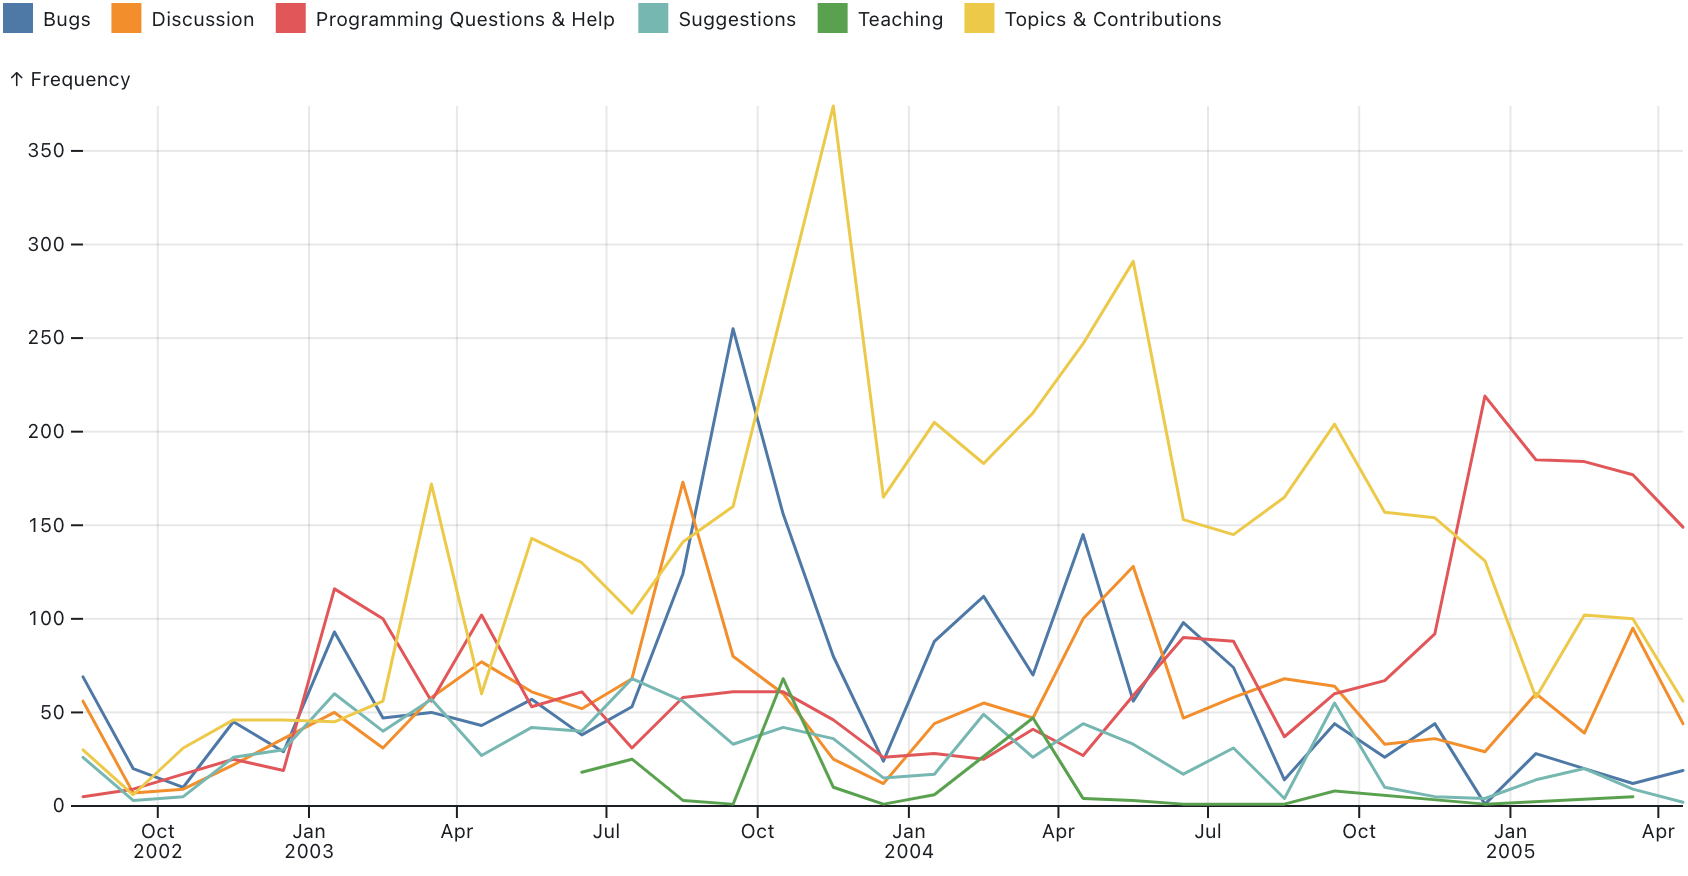
\includegraphics[width=1\textwidth]{alpha-forums-activity.png} 
    % \includesvg[pretex=\sffamily\fontsize{5.58pt}{8pt}\selectfont, width=0.6\textwidth]{images/alpha-forums-activity.svg}
    \caption{Forums activity}
    \label{fig:forum-activity}  
  \end{figure}